% enable this to activate the version for PRINT
% disable this to make the pdf symmetric and without white pages
% => asymmetric alternating left/right margins
% \newcommand*{\printversion}{}%

%% | ---------------- document meta information --------------- |

\newcommand{\Author}{Petr Kučera}
\newcommand{\Department}{Department of Cybernetics}
\newcommand{\Supervisor}{Ing. David Čapek}
\newcommand{\SupervisorSpecialist}{Ing. My Specialist, Ph.D.}
\newcommand{\Programme}{Cybernetics and Robotics}
\newcommand{\Field}{Artificial Intelligence and Biocybernetics} % todo ???
%\newcommand{\Title}{Rigorous Evaluation of Large-scale\\[0.5em]Mapping and Localization Systems\\[0.5em]on High-fidelity Synthetic Datasets}
\newcommand{\Title}{Rigorous Evaluation of Large-scale\\[0.3em]Mapping and Localization Systems\\[0.3em]on High-fidelity Synthetic Datasets}
\newcommand{\Keywords}{Unmanned Aerial Vehicles, Flight Forge Simulator, Procedural Environment Generation, Unreal Engine 5, Segmentation, Binary Mask Processing, Spline Generation, Mapping Validation}
\newcommand{\KlicovaSlova}{Bezpilotní prostředky, Flight Forge simulátor, Procedurální generace prostředí, Unreal Engine 5, Segmentace, Zpracování binárních masek, Generace křivek, Validace mapování}
\newcommand{\Year}{2025}
\newcommand{\Month}{April}
\newcommand{\Date}{\Month~\Year}
\newcommand{\Location}{Prague}

%% | ---------------------- configuration --------------------- |

% most of the configuration stuff happens here
\input{src/document_setup.tex}

%% | ---------------------- the contents ---------------------- |

\begin{document}

% this will prevent unwanted line overflows
% http://latexref.xyz/_005cfussy-_0026-_005csloppy.html
\sloppy

\pagenumbering{roman}

%% --------------------------------------------------------------
%% |                         Title page                         |
%% --------------------------------------------------------------

\input{src/title}

% set up the page style for the "intro" pages
\pagestyle{plain}

%% --------------------------------------------------------------
%% |                       Acknowledgments                      |
%% --------------------------------------------------------------

\conditionalClearPage

%!TEX root = ../main.tex

\section*{Acknowledgments}


\vspace{2.5cm}


%% --------------------------------------------------------------
%% |                         Assignment                         |
%% --------------------------------------------------------------

\conditionalClearPage

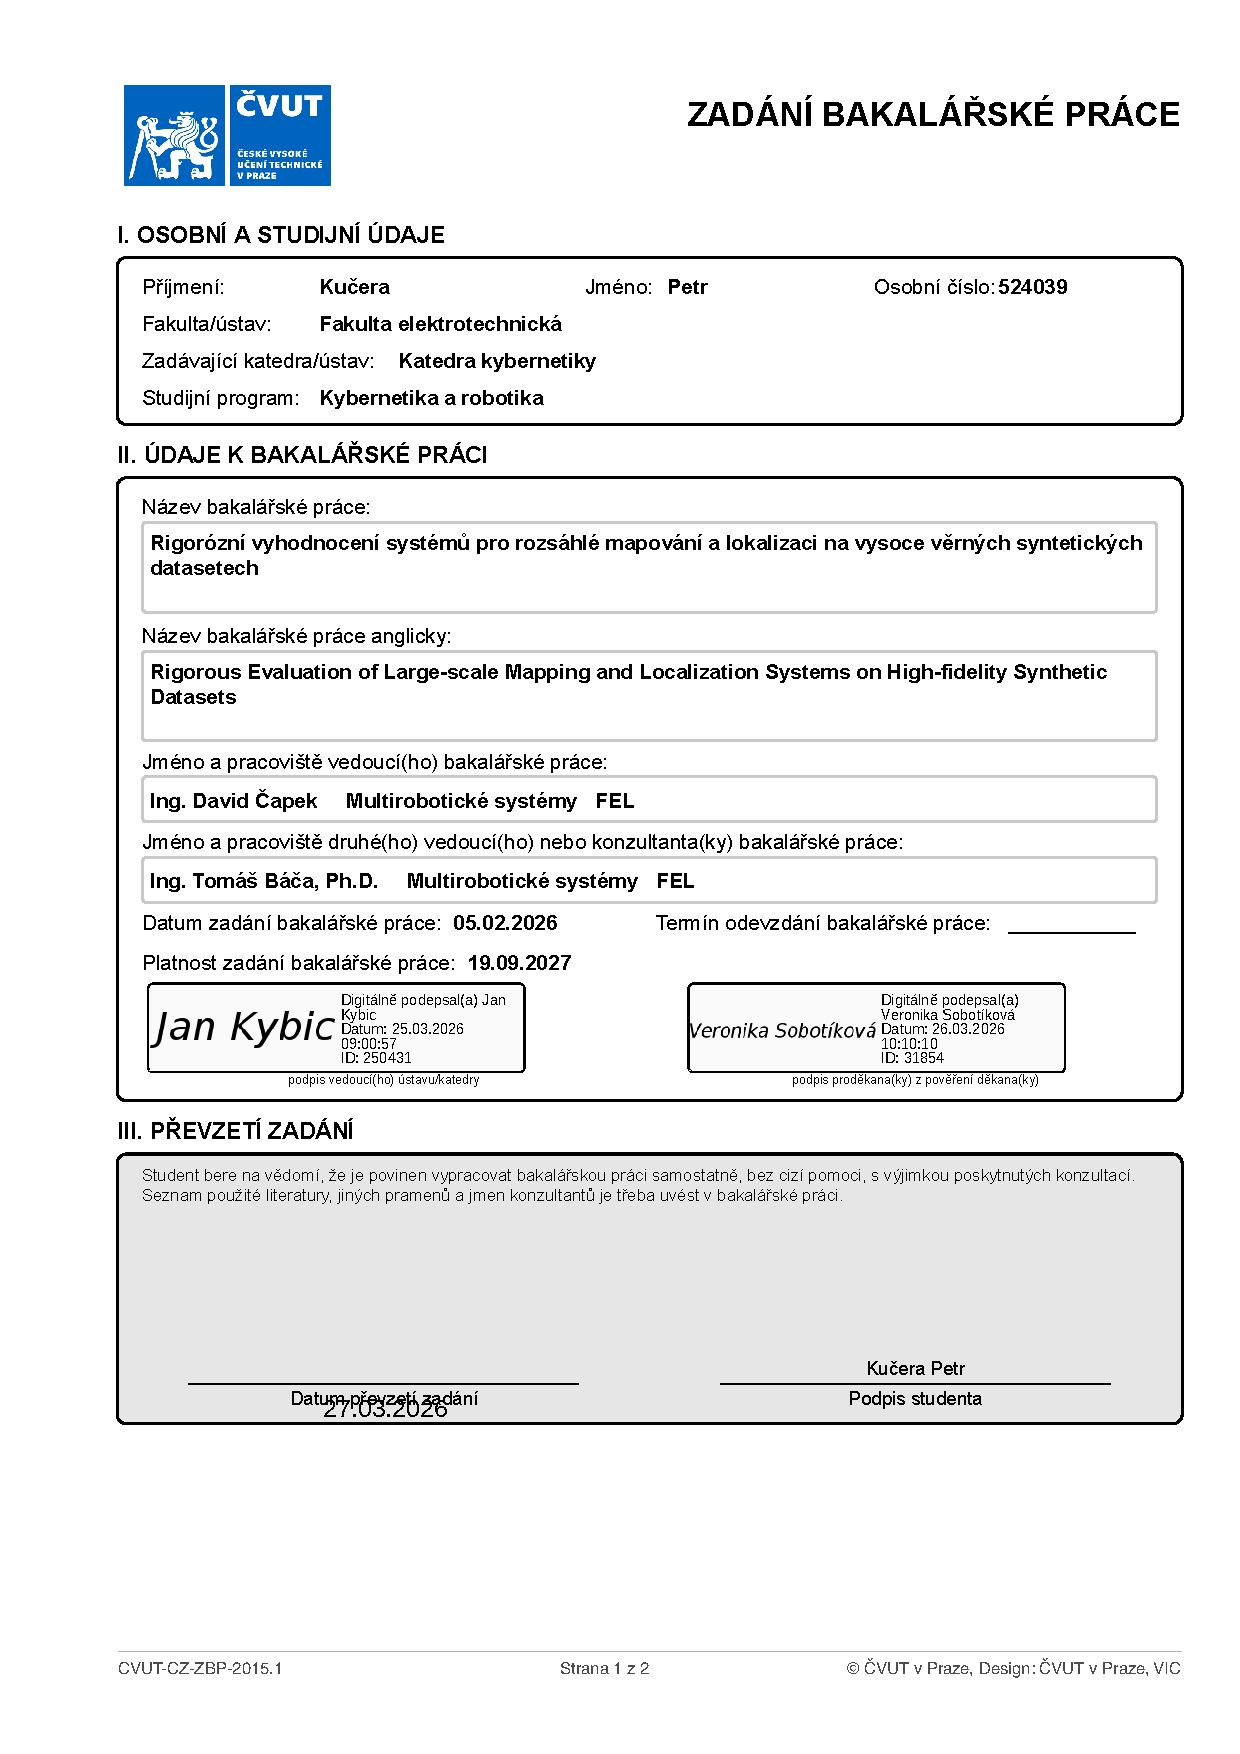
\includepdf[pages=-]{src/assignment.pdf}

%% --------------------------------------------------------------
%% |                         Declaration                        |
%% --------------------------------------------------------------

\conditionalClearPage


\includepdf[pages=-]{src/Declaration.pdf}

%% --------------------------------------------------------------
%% |                          Abstracts                         |
%% --------------------------------------------------------------

\conditionalClearPage

%!TEX root = ../main.tex

\begin{changemargin}{0.8cm}{0.8cm}

~\vfill{}

\section*{Abstract}
\vskip 0.5em

Virtual environments are increasingly used in simulation, testing, and training scenarios. However, manual creation of such environments is a time-consuming process, especially when the environments are large outdoor worlds. This thesis focuses on a semi-automatic method for creating outdoor procedural environments while preserving user control over the generation process.

The proposed method uses height maps and segmentation images as the basis for environment generation inside Unreal Engine~5. A height map is used to create the landscape, while segmentation images are processed into binary masks. From these masks, skeletons and contours are extracted. Skeletons are used to generate roads and rivers, while contours are used to generate lakes and biome regions. Biome generation is implemented using the Unreal Engine~5 PCG Biome Core plugin.

Four worlds were generated using the proposed method. These worlds were then used to create datasets with the Flight Forge simulator and on them selected mapping frameworks were evaluated. The created datasets can be used for testing localization, mapping, LiDAR odometry and visual odometry. Additionally, if the generated environments are based on satellite imagery, the resulting datasets can also be compared with corresponding real-world locations.

\vskip 1em

{\bf Keywords} \Keywords

\vskip 2.5cm

\end{changemargin}


\conditionalClearPage

%!TEX root = ../main.tex

\begin{changemargin}{0.8cm}{0.8cm}

~\vfill{}

\section*{Abstrakt}
\vskip 0.5em

\sloppy
Výzkum na poli autonomních bezpilotních prostředků (UAV) se stal významným oborem mobilní robotiky.

1-2 věty problem definition
3-4 věty na metodologii - nějak vymyslíš :D
- results - datasets a otestování na mapping frameworks -> dataset pro lokalizaci, mapování, lidarové odometrie, vizuální odometrie, prior map usage (ze satelitního snímku se udělá svět a pak porovná s realitou)

\vskip 1em

{\bf Klíčová slova} \KlicovaSlova

\vskip 2.5cm

\end{changemargin}


%% --------------------------------------------------------------
%% |                        Abbreviations                       |
%% --------------------------------------------------------------

\conditionalClearPage

\begin{changemargin}{0.8cm}{0.8cm}

~\vfill{}

\section*{Abbreviations}

% this will print only the used abbreviations
\input{src/abbreviations.tex}

\vskip 2.5cm

\end{changemargin}

\conditionalClearPage

%% --------------------------------------------------------------
%% |                      Table of contents                     |
%% --------------------------------------------------------------

\tableofcontents

\listoffigures % List of figures

% \listoftables % List of tables (maybe remove)

\conditionalClearPage

% set up the full page style with normal page numbering
\pagestyle{full}
\pagenumbering{arabic}

%% --------------------------------------------------------------
%% |                        introduction                        |
%% --------------------------------------------------------------

%!TEX root = ../main.tex

\chapter{Introduction\label{chap:introduction}}

Virtual environments are increasingly used in simulation, testing, and training scenarios. In the context of \ac{UAV}, simulated worlds make it possible to test navigation, perception, and decision-making methods in controlled conditions before deploying them in the real world. For such simulations to be useful, the environment should contain meaningful spatial structure. Virtual environments can be categorized into indoors and outdoors environments.

Indoors environments are more difficult to generate without the usage of \ac{AI}. For example creating realistic, and more importantly believable, apartment only by using procedural generation algorithms can not be easily achieved. On the other hand, when the neural network is trained on data regarding placement of props in indoors environments, creating non-random scene as a apartment can be done. 

Outdoors environments are easier to produce via procedural generation algorithms. Many popular games utilize these algorithms to create realistic and believable open world environments. Usage of \ac{AI} in this area is mainly in pre-generation step, or while generating complex sections such as cities, as the usage of standard algorithms is computationally less expensive and results do not differ as much. 

Creating outdoor environments manually is a time-consuming process. Elements such as terrain, roads, rivers, lakes, and biome areas often have to be placed consistently with the intended layout of the scene. When created manually, this process requires a significant amount of repetitive work and can become difficult to manage for larger environments.

One way to reduce this workload is to use input data that already describes the desired structure of the environment. Height maps can define the terrain elevation, while segmentation images can describe the placement of different environmental features such as roads, rivers, lakes, forests, or other biome types. However, these image-based representations cannot be used directly as editable objects inside a real-time 3D engine. They first need to be processed and converted into engine-specific structures.

This thesis focuses on the design and implementation of an Unreal Engine plugin that automates part of this process. The plugin uses height maps and segmentation images to generate the initial structure of a virtual environment. Opposed to autonomous procedural generation this work focuses to giving the user of this plugin the ability to adjust any step of the generation pipeline. 

By converting image-based input data into editable Unreal Engine objects, the proposed plugin reduces the amount of manual work required to build the simulation environment while preserving user control over the final result. Such environments can then be used as a basis for simulation scenarios or generation of datasets for evaluating mapping and localization methods.

The implemented plugin is designed with the Flight Forge~\cite{bk_flight_forge} simulation workflow in mind. Its purpose is to support the creation of high-fidelity environments that can later be used for robotic simulation and dataset generation. In this context, the generated worlds may serve as a source of sensor data, such as RGB images or \ac{LiDAR} measurements, together with corresponding ground-truth information.

\section{Related Works}

% todo přepsat toto aby to více souviselo s tím co píšu dole?

Recent advances in development of artificial intelligence have shown promising results regarding generation of unique environments suitable for robotic simulations. Many works specialize in generating environments completely randomly to ensure their uniqueness while other focus on creating real-life environments from publicly available data, such as satellite imagery. 

% todo nějak to co je pod tímto rozdělit do subsekcí 
% todo nějak zpřeházet pořadí?

Pipeline of the manual creation of different outdoor environments inside Unreal Engine~5 was proposed in this paper~\cite{bk_seg_gen_ue5}. This approach uses hand made landscape and hand drawn RGB biome mask as basis for environment generation. This pipeline does not take road, river, lake or city creation into account, limiting the resulting datasets.

More automated process of generating realistic environment using satellite imagery was proposed in this paper~\cite{bk_satellite_ue5}. Converted satellite data into height map and color mask are used in automated landscape generation with biomes. This approach is highly depended on precision of provided satellite data and user can not create completely random environments. % todo trochu eh

Procedural urban environment generation proposed in these paper~\cite{bk_simworld_robotics_urban},\cite{bk_procedural_urban} is used to train deep neural networks to navigate in such complex environments. Proposed algorithms in both papers follow similar pipeline: road generation, building generation and street element generation. 

Another proposed generator of synthetic datasets is Infinigen~\cite{bk_infinigen_outdoor}. It is a generator that can create infinitely natural environments. As this generator is build on top of Blender, % todo reference here?
resulting photo-realistic environments comes only as renders, not fully explorable worlds. 

% ^^^ spíše světy | vvv spíše indoor - odstavec pod tím je takovej segway :D

However Infinigen generator is limited to natural scenes. To overcome this limitation, Infinigen Indoors~\cite{bk_infinigen_indoor} was created. In works similarly as Infinigen in creating photo-realistic renders. To create completely unique indoors environments without need of many different props, this generator has the ability to procedurally generate them.

Thanks to the advanced \ac{LLM} and \ac{VLM} generation of realistic environments are possible from simple prompts. Proposed solution in this paper~\cite{bk_3d_generalist} is by utilizing combination of \ac{LLM}, to process the input prompt, and \ac{VLM}, to generate visually appealing environment. 



\section{Mathematical Notation}

\begin{table*}[!h]
  \scriptsize
  \centering
  \noindent\rule{\textwidth}{0.5pt}
  \begin{tabular}{lll}
    $\mathbf{x}$, $\bm{\alpha}$ & vector, pseudo-vector, or tuple\\
    $\mathbf{\hat{x}}$, $\bm{\hat{\omega}}$& unit vector or unit pseudo-vector\\
    $\mathbf{\hat{e}}_1, \mathbf{\hat{e}}_2, \mathbf{\hat{e}}_3$ & elements of the \emph{standard basis} \\
    $\mathbf{X}, \bm{\Omega}$ & matrix \\
    $\mathbf{I}$ & identity matrix \\
    $x = \mathbf{a}^\intercal\mathbf{b}$ & inner product of $\mathbf{a}$, $\mathbf{b}$ $\in \mathbb{R}^3$\\
    $\mathbf{x} = \mathbf{a}\times\mathbf{b}$ & cross product of $\mathbf{a}$, $\mathbf{b}$ $\in \mathbb{R}^3$\\
    $\mathbf{x} = \mathbf{a}\circ\mathbf{b}$ & element-wise product of $\mathbf{a}$, $\mathbf{b}$ $\in \mathbb{R}^3$ \\
    $\mathbf{x}_{(n)}$ = $\mathbf{x}^\intercal\mathbf{\hat{e}}_n$ & $\mathrm{n}^{\mathrm{th}}$ vector element (row), $\mathbf{x}, \mathbf{e} \in \mathbb{R}^3$\\
    $\mathbf{X}_{(a,b)}$ & matrix element, (row, column)\\
    $x_{d}$ & $x_d$ is \emph{desired}, a reference\\
    $\dot{x}, \ddot{x}, \dot{\ddot{x}}$, $\ddot{\ddot{x}}$ & ${1^{\mathrm{st}}}$, ${2^{\mathrm{nd}}}$, ${3^{\mathrm{rd}}}$, and ${4^{\mathrm{th}}}$ time derivative of $x$\\
    $x_{[n]}$ & $x$ at the sample $n$ \\
    $\mathbf{A}, \mathbf{B}, \mathbf{x}$ & LTI system matrix, input matrix and input vector\\
    \emph{SO(3)} & 3D special orthogonal group of rotations\\
    \emph{SE(3)} & \emph{SO(3)}~$\times~\mathbb{R}^3$, special Euclidean group\\
  \end{tabular}
  \noindent\rule{\textwidth}{0.5pt}
  \caption{Mathematical notation, nomenclature and notable symbols.}
  \label{tab:mathematical_notation}
\end{table*}


%% --------------------------------------------------------------
%% |						 methodology						|
%% --------------------------------------------------------------

\chapter{Methodology}

% todo změnit názvy jako unreal engine features s přesnou definicí, cotoe

\section{Binary Mask Processing}

\subsection{Binary Mask Creation}

% todo redo this VVVV (přidat vzorec a tak?)

A segmentation image is converted into a binary mask by selecting all pixels whose color lies within a specified range. This range can be adjusted by the user to obtain finer control over binary mask creation.

The result is a binary image in which white pixels, referred to as foreground, are assigned the value true, while black pixels, referred to as background, are assigned the value false. We refer to clusters of white or black pixels as regions. 

% todo obrázek segmentace -> masky -> smoothnuté masky

\subsection{Euclidean Distance Transform}

The Euclidean distance transform, referred to as EDT, assigns to each pixel the Euclidean distance to the nearest pixel of a specified set. This can be used for extracting widths from binary masks.

In our implementation, the cost function $f$ is chosen so that distances are computed from foreground pixels to the nearest background pixel. This is determined by which pixels are assigned the values $0$ and $\infty$ in the cost function.

This process can be generalized to transform a cost function on a grid using spatial information~\cite{bk_edt}, such as using distance function other than Euclidean, or $n$-dimensional grids.

We define cost function as $f(q)$:
\begin{equation}
	f(q) =
	\begin{cases}
		\infty & \text{if } q \text{ is a foreground pixel}, \\
		0 & \text{otherwise},
	\end{cases}
\end{equation}
where $q$ is a pixel of the binary mask. The distance transform of $f$ is denoted by $\mathcal{D}_f$ and defined as
\begin{equation}
	\mathcal{D}_f(p) = \min_{q\in \mathcal{G}}\left(d(p,q) + f(q)\right),
\end{equation}
where $\mathcal{G}$ is the grid representing the binary mask, $p \in \mathcal{G}$, and $d(p,q)$ is a distance function.If $d(p,q)$ is chosen as Euclidean distance, then $\mathcal{D}_f$ is called the Euclidean distance transform.

Applying EDT to the binary mask yields a distance field. The value at each element of the distance field is the distance from the corresponding pixel in the binary mask to the nearest background pixel. This can be seen in definition of function $f(q)$, where its value for black pixels is zero, meaning $\mathcal{G}$ computes distance of a white pixel to a black pixel. Consequently, the value of every background pixel in this field is $0$.

% todo obrázek binarymask -> hodnoty EDT (+ nekonečna?) - tedy distance field

In our application, this algorithm is used to extract the widths of roads or rivers by computing EDT of foreground pixels. These widths can then be converted to approximate real-world measurements. The precision of this approach depends on the accuracy and resolution of the binary mask.

\subsection{Signed Distance Field}

Signed distance field, or SDF, is a field in which the value corresponding to each pixel of binary mask represents the distance from that pixel to the nearest boundary between foreground and background region. Unlike the unsigned distance field, the SDF stores meaningful values on both sides of the foreground boundary. To differentiate between the two colors, we denote the distances of background pixels as negative.

First we define distance transform $\mathcal{D}_g$ for background pixels by inverting the cost function, so we compute distances of black pixel to a white pixel. The cost function $g(q)$ is
\begin{equation}
	g(q) =
	\begin{cases}
		\infty & \text{if } q \text{ is a background pixel}, \\
		0 & \text{otherwise},
	\end{cases}
\end{equation}
where $q$ is a pixel of the binary mask. The distance transform of $g$ is denoted by $\mathcal{D}_g$ and defined as
\begin{equation}
	\mathcal{D}_g(p) = - \min_{q\in \mathcal{G}}\left(d(p,q) + g(q)\right),
\end{equation}
where $\mathcal{G}$ is the grid representing the binary mask, $p \in \mathcal{G}$, and $d(p,q)$ is the Euclidean distance.

Signed distance field has the same dimensions as the initial binary mask. The SDF value $v$ at pixel $p$ is defined as the sum of these two distance transforms
\begin{equation}
	v = \mathcal{D}_f(p) + \mathcal{D}_g(p),
\end{equation}
where $p$ is a pixel on binary mask. When $p$ is a foreground pixel, $\mathcal{D}_f(p)$ is positive, while $\mathcal{D}_g(p) = 0$. Conversely, when $p$ is a background pixel, $\mathcal{D}_f(p)=0$ and $\mathcal{D}_g(p)$ in a negative value. 

% todo obrázek binarymask -> hodnoty SDF na té samé masce jako nahoře

\subsection{Binary Mask Smoothing}

Binary mask smoothing is achieved by applying Gaussian blur to the computed signed distance field. The blurred field is then classified by a threshold. Values above a this threshold are classified as foreground, while the remaining values are classified as background. When applied to very thin foreground regions, this process may disrupt their continuity.

Gaussian function for two dimensions is defined as
\begin{equation}
	G(x,y) = \frac{1}{2\pi\sigma^2}\exp\left(-\frac{x^2 + y^2}{2\sigma^2}\right),
\end{equation}
where parameter $\sigma$ determines the blur strength. Increasing $\sigma$ results in stronger smoothing, while decreasing produces weaker smoothing.

To blur an image $I(x,y)$ we compute its convolution with Gaussian function
\begin{equation}
	I_\text{blurred}(x,y) = (I * G)(x,y) = \sum_u\sum_v I(x-u, y-v)G(u,v).
\end{equation}
In discrete implementation we use kernel of size $(2R + 1)\times(2R+1)$, where $R$ is a radius generally chosen as
\begin{equation}
	R = \max\left(1, \lceil 3 \sigma \rceil\right),
\end{equation}
because the value of Gaussian function outside the interval $\left[-3\sigma, +3\sigma\right]$ is relatively small.

If we use computed SDF of binary mask as our image, then we get resulting blurred SDF as
\begin{equation}
	\text{SDF}_\text{blurred}(x,y) = \sum_{u = -R}^R \sum_{v = -R}^R \text{SDF}(x - u, y - v)G(u,v),
\end{equation}
where $\text{SDF}(x,y)$ is an element of SDF at $x$ and $y$ coordinate, and $0\leq x < \text{width}$ and $0 \leq y < \text{height}.$

The user is given option to adjust both Gaussian blur parameter $\sigma$ the threshold value. Increasing the threshold erodes the resulting mask, whereas decreasing it expands the foreground region.

% todo obrázek -> smooth -> grown -> eroded

\section{Topology Extraction from Binary Masks} % todo maybe toto přejmenovat idk man

\subsection{Binary Mask Skeletonization}

Thinning of a binary mask, referred to as skeletonization, is a process of removing boundary pixels of a foreground region while maintaining their basic structure, general shape and connectivity. For algorithms used to create binary mask skeleton used for this application, we need to ensure satisfaction of certain criteria:
\begin{itemize}
	\item The resulting line should be 1 pixel wide with no redundant pixels
	\item Connectivity of individual components must be preserved
	\item The skeleton should be approximately centered with respect to the local thickness of the component.
	\item There should not be substantial gap between skeleton and edge of binary mask, if the foreground region is touching the side.
\end{itemize}

Many thinning algorithms have been proposed for various applications, one of the popular ones are Guo-Hall algorithm and Zhang-Suen algorithm~\cite{bk_zhang_suen}. Their main advantage is their ability to be parallelized, but both of them do not guarantee desired 1-pixel width without some additional post-processing. A different algorithm was selected~\cite{bk_jain_himanshu}, which is sequential and guarantees skeleton with no redundant pixels and 1-pixel width. 

% todo IMAGE GUO-HALL X ZHANG-SUEN X JAIN-KUMAR

This algorithm works by performing passes in all four directions and sequentially removes redundant pixels until only the skeleton remains. This results in the skeleton being offset by 1 pixel from center, but this error is insignificant and does not negatively affect the final result. 

Additional advantage to its 1-pixel width, is that if foreground region of binary mask is touching image boundary, the algorithm will not create substantial gap between first point of the skeleton and side of the image. For example Zhang-Suen algorithm does not have this feature and it can result in unrealistic rivers or roads.

% todo obrázek s edge skeletonem

% todo pseudo kód?

Disadvantage of skeletonization algorithms is that they are sensitive to binary mask "corners". As the algorithm creates skeleton to be in the middle, when some section of the foreground region is sharper, it can create branch towards this corner. This can be resolved by smoothing the binary mask before performing skeletonization.

% todo ukázat ten branch ze skeletonu
% todo ukázat ten brach ze skeletonu po smoothování

\subsection{Contour Extraction of Area Features}

Extracting contours of binary mask foreground region is used for creating features that fill area, such as biomes or lakes. 

Used algorithm cycles through every pixel of binary mask. If the pixel is black, that means in background, we skip it. If the pixel is white, in foreground, we count how many 4-neighbors are black and if there are any, we mark this pixel as contour. Pixels that are 4-neighbors are the pixels directly above, below, left or right of the initial pixel.

This algorithm skips foreground pixels along the edges of binary mask, as there are no background pixels. To create edge contour we count pixels that are outside the binary mask bounds as background.

% todo obrázek s validní contůrou

This algorithm, although simple, reliably detects contours. There are a few scenarios where strictly 1-pixel width of the contours is not ensured. These scenarios are hard to resolve by algorithm as their outcome can rapidly change the shape or size of the contours. We decided to leave the resolution of these situations to user by giving them tools for manual edit.

% todo obrázek s nevalidní contůrou

% Caption setup for algorithm 
\captionsetup[algorithm]{
	labelfont=bf,
	justification=raggedright,
	singlelinecheck=false
}

\section{Polyline Creation from Topological Pixels}

A polyline is represented os an ordered list of points $\mathbf{P}_0, \mathbf{P}_1, ..., \mathbf{P}_n$ where each consecutive pair of points $\left(\mathbf{P}_i, \mathbf{P}_{i+1}\right)$, where $i = 0,1,...,n$, defines one line segment. In this way, the polyline forms a connected piecewise curve composed of the segments
\begin{equation*}
	(\mathbf{P}_0, \mathbf{P}_1), (\mathbf{P}_1, \mathbf{P}_2), ..., (\mathbf{P}_{n-1}, \mathbf{P}_n).
\end{equation*}
Since the points are ordered, the connectivity of the polyline is given implicitly by their order in the list. 

Special case of polyline is a closed polyline. A polyline is considered closed if its first and last point are identical,
\begin{equation}
	\mathbf{P}_0 = \mathbf{P}_n.
\end{equation}

% todo ukázka polyline na obrázku xd

\subsection{Pixel Classification}

To create polylines we need to classify topological pixels, determining whether a pixel is an endpoint or a junction. We use a simple classification method based on counting the number of foreground pixels in the 8-neighborhood of the examined pixel.

If the number of foreground neighbors is one, the pixel is classified as an endpoint, since it is connected to only one neighboring pixel. If the number is two, the pixel is considered a regular polyline pixel connecting two neighboring pixels.

% todo obrazek endpointu, normální, junction, a abomination jako plateau or other.

A junction pixel has three or more foreground neighbors, although in typical cases it has exactly three. If four or more foreground neighbors are present, this may indicate a more complex local structure, such as a plateau or another shape that can complicate polyline extraction.


\subsection{Polyline Tracing Algorithm}

The extracted topology, whether obtained from a binary mask skeleton or from a contour, is still represented as an unordered set of foreground pixels in the image grid. For subsequent processing, such as simplification or spline construction, this discrete representation must be converted into an ordered geometric form.

The goal of the tracing algorithm is therefore to convert the extracted topology pixels into one or more ordered polylines that collectively cover all foreground pixels of the topology. To achieve this, the algorithm uses the previously classified endpoint and junction pixels together with a visited map. The visited map stores whether a foreground pixel has already been assigned to a traced polyline, which prevents the same branch from being processed repeatedly. Junction pixels require special treatment, because a single junction may belong to multiple output polylines.

The tracing is divided into three steps. First, all branches starting at endpoints are traced until another endpoint or a junction is reached. Second, the remaining branches connecting pairs of junctions are traced. Finally, any still unvisited foreground pixels are assumed to belong to closed contours and are processed separately. This ordering is important, because endpoint-based branches are the least ambiguous, while closed contours can only be identified reliably after all open branches have already been removed.

\subsection{Tracing from Endpoint to Junction or Endpoint}

The first step constructs a polyline starting at an endpoint and following the topology until either another endpoint or a junction is reached. This case corresponds to a branch with a well-defined starting point, and it is therefore the most straightforward tracing scenario.

The algorithm starts by inserting the selected endpoint into the polyline and marking it as visited. It then repeatedly examines the 8-neighborhood of the current pixel and selects the next foreground pixel that has not yet been visited. On the newly found pixel, one of the three following actions is performed:
\begin{itemize}
	\item If the pixel is an endpoint, it is marked as visited, added to the polyline and the branch is complete.
	\item If the pixel is an junction, the branch is also terminated, but the pixel is not marked as visited.
	\item If the pixel is regular topology pixel, it is marked as visited, appended to the polyline, and the tracing continues from that location.
\end{itemize}

When more than one valid foreground neighbor is available, endpoint or junction candidates are prioritized over regular foreground pixels. Among such candidates, the closest one is selected using Manhattan distance. This additional selection rule improves continuity of the resulting polyline and reduces the occurrence of short redundant segments or incorrect local detours that may otherwise appear in discrete pixel topology.

{
	\captionof{algorithm}{Polyline from Endpoint to Junction or Endpoint algorithm}
	\begin{algorithmic}[1]
		\Procedure{Endpoint\_to\_junction\_or\_endpoint}{$\textit{starting\_endpoint},\textit{visited}$}
		\State $\textit{queue} \gets \text{initialize queue}$
		\State $\textit{polyline} \gets \text{initialize empty polyline}$
		\State
		\State $\textit{queue}\text{.add(}\textit{starting\_endpoint}\text{)}$
		\While{$\textit{queue}$ is not empty}
		\State $\textit{point} \gets \textit{queue}\text{.pop()}$ 
		\State
		\State $\textit{visited}\text{[}\textit{ point }\text{]} = \text{true}$
		\State $\textit{polyline}\text{.add(}\textit{point}\text{)}$
		\State
		\State $\textit{best\_endpoint\_or\_junction}\gets\textbf{ select from neighbors of }\textit{point}$
		\If{$\textit{best\_endpoint\_or\_junction}\text{ exists}$}
		\State $\textit{polyline}\text{.add(}\textit{best\_endpoint\_or\_junction}\text{)}$
		\State
		\Return $\textit{polyline}$
		\EndIf
		\State
		\For {$\textit{neighbor}\textbf{ from }\textit{neighbors}\textbf{ of }\textit{point}$}
		\If{$\textit{neighbor}\text{ is foreground} \textbf{ and } \text{not }\textit{visited}\text{[}\textit{ neighbor }\text{]}$}
		\State $\textit{queue}\text{.add(}\textit{neighbor}\text{)}$
		\State $\textbf{break}$
		\EndIf
		\EndFor
		\EndWhile
		
		\State
		\State
		\Return $\textit{polyline}$
		\EndProcedure
	\end{algorithmic}
}

\subsection{Tracing from Junction to Junction}

After all branches with endpoint start vertices have been processed, some foreground pixels may still remain unvisited. In a skeleton topology, these remaining pixels are typically expected to form branches connecting one junction to another. Unlike the previous case, a junction can have multiple outgoing branches, and therefore one starting junction may produce several output polylines.

For this reason, the algorithm considers each unvisited foreground neighbor of the starting junction separately. For every such neighbor, a new polyline is initialized with the starting junction as its first point. If the selected neighbor is itself a junction, the resulting branch consists only of a direct connection between two adjacent junctions, and the tracing for that branch ends immediately.

Otherwise, the neighbor is treated as the first regular pixel of a new branch. The tracing then proceeds in the same way as in the endpoint case. Regular pixels are appended to the polyline and marked as visited, while the first encountered junction terminates the current branch. The starting junction is marked as visited before the traversal begins, but terminal junctions are not marked during branch termination, since they may also participate in other junction-to-junction branches.

As in the previous step, a junction candidate found in the current 8-neighborhood is prioritized over regular foreground pixels. If more such candidates exist, the closest one is selected according to Manhattan distance. This makes the tracing more stable in ambiguous local configurations and helps preserve the intended branch structure of the topology.

{
	\captionof{algorithm}{Polyline from Junction to Junction algorithm}
	\begin{algorithmic}[1]
		\Procedure{Junction\_to\_junction}{$\textit{starting\_junction},\textit{visited}$}
		\State $\textit{polyline\_list} \gets \text{initialize empty polyline list}$
		\State
		\State $\textit{visited}\text{[ }\textit{starting\_junction}\text{ ]}$ = true
		\State
		\For {$\textit{starting\_neighbor}\textbf{ from }\textit{neighbors}\textbf{ of }\textit{starting\_junction}$}
			\If{$\textit{visited}\text{[ }\textit{starting\_neighbor}\text{ ]}$ } 
				\State $\textbf{continue}$
			\EndIf
			\State
			\State $\textit{queue} \gets \text{initialize queue}$
			\State $\textit{polyline} \gets \text{initialize empty polyline}$
			\State $\textit{polyline}\text{.add(}\textit{starting\_junction}\text{)}$
			\State
			\State $\textit{queue}\text{.add(}\textit{starting\_neighbor}\text{)}$
			\While{$\textit{queue}$ is not empty}
				\State $\textit{point} \gets \textit{queue}\text{.pop()}$ 
				\State
				\If{$\textit{point}\textbf{ is junction}$}
					\State $\textit{polyline}\text{.add(}\textit{point}\text{)}$
					\State $\textbf{break}$
				\EndIf
				\State
				\State $\textit{visited}\text{[}\textit{ point }\text{]} = \text{true}$
				\State $\textit{polyline}\text{.add(}\textit{point}\text{)}$
				\State
				\State $\textit{best\_endpoint\_or\_junction}\gets\textbf{ select from neighbors of }\textit{point}$
				\If{$\textit{best\_endpoint\_or\_junction}\text{ exists}$}
					\State $\textit{polyline}\text{.add(}\textit{best\_endpoint\_or\_junction}\text{)}$
					\State $\textbf{break}$
				\EndIf
				\State
				\For {$\textit{neighbor}\textbf{ from }\textit{neighbors}\textbf{ of }\textit{point}$}
					\If{$\textit{neighbor}\text{ is foreground} \textbf{ and } 		\text{not }\textit{visited}\text{[}\textit{ neighbor }\text{]}$}
						\State $\textit{queue}\text{.add(}\textit{neighbor}\text{)}$
						\State $\textbf{break}$
					\EndIf
				\EndFor
			\EndWhile
			\State
			\State $\textit{polyline\_list}\text{.add(}\textit{polyline}\text{)}$
		\EndFor
		\State
		\State
		\Return $\textit{polyline\_list}$
		\EndProcedure
	\end{algorithmic}
}

\subsection{Tracing from Closed Contour}

After the previous two steps, all open branches are expected to have been removed from consideration. Any remaining unvisited foreground pixels are therefore assumed to belong to closed polylines with no endpoints and no junctions. Such cases occur most commonly when tracing contours of foreground regions rather than skeleton centerlines.

The algorithm begins by selecting any unvisited foreground pixel as the starting point of a new polyline. This point is appended to the polyline, marked as visited, and used as the initial tracing position. The algorithm then repeatedly searches the 8-neighborhood for another unvisited foreground pixel and continues the traversal until no such neighbor exists.

Because this case does not contain endpoints or junctions, no special termination pixel is expected during the traversal. Instead, the tracing ends only when the algorithm returns to a state in which the current point has no unvisited foreground neighbor. At that moment, the entire closed contour has been traversed. To represent closure explicitly in our implementation, the initial starting point is appended to the polyline once more, so that the first and last point of the resulting ordered list are identical.

{
	\captionof{algorithm}{Polyline from Closed Contour algorithm}
	\begin{algorithmic}[1]
		\Procedure{Closed\_contour\_to\_polyline}{$\textit{starting\_point},\textit{visited}$}
		\State $\textit{queue} \gets \text{initialize queue}$
		\State $\textit{polyline} \gets \text{initialize empty polyline}$
		\State
		\State $\textit{queue}\text{.add(}\textit{starting\_point}\text{)}$
		\While{$\textit{queue}$ is not empty}
			\State $\textit{point} \gets \textit{queue}\text{.pop()}$ 
			\State
			\State $\textit{visited}\text{[}\textit{ point }\text{]} = \text{true}$
			\State $\textit{polyline}\text{.add(}\textit{point}\text{)}$
			\State
			\For {$\textit{neighbor}\textbf{ from }\textit{neighbors}\textbf{ of }\textit{point}$}
				\If{$\textit{neighbor}\text{ is foreground} \textbf{ and } \text{not }\textit{visited}\text{[}\textit{ neighbor }\text{]}$}
					\State $\textit{queue}\text{.add(}\textit{neighbor}\text{)}$
					\State $\textbf{break}$
				\EndIf
			\EndFor
		\EndWhile
		\State
		\State $\textit{polyline}\text{.add(}\textit{starting\_point}\text{)}$
		\State 
		\Return $\textit{polyline}$
		\EndProcedure
	\end{algorithmic}
}

\subsection{Edge Cases}

There are several edge cases that can be handled by the previously described algorithms, but not in an optimal way. In this application, which also relies heavily on user input, we decided not to handle these cases automatically, as doing so may produce unwanted results. Instead, we provide tools that allow the user to resolve such cases manually, for example by stitching two or more polylines together or by closing a polyline.

Examples of such edge cases include the previously mentioned junction plateaus and L-shaped corners. Although the algorithm can process these cases, it may create redundant line segments or unnecessary connections. Another encountered edge case arises when a 2-pixel-wide contour is created from a foreground region that is too thin. This may result in many short line segments and in a polyline that is not closed.

% todo obrázek L, plateau atd a jak to algoritmus řeší -> tedy asi barvevné spojnice středů?

% todo obrázek rozsypané kontůry

\section{Polyline Post-processing}

\subsection{Polyline Stitching Algorithm}

\subsection{Polyline Simplification Using Douglas--Peucker Algorithm} % todo check jména, not sure about it :D

\section{Spline Construction from Polylines}

\subsection{Hermite and B\'ezier Curve Representations}

In our implementation, we chose to represent splines as a sequence of cubic B\'ezier curves rather than as Hermite curves, which are used internally by Unreal Engine~5. The main reason for this choice is that B\'ezier curves are more convenient for the algorithms introduced later in this chapter. At the same time, a cubic B\'ezier curve can be converted to a Hermite representation in a straightforward manner.

A cubic B\'ezier curve $\mathbf{B}(t)$ is defined by two end points, $\mathbf{P}_0$ and $\mathbf{P}_3$, and two control points, $\mathbf{P}_1$ and $\mathbf{P}_2$. It is given by
\begin{equation}
	\mathbf{B}(t) = (1 - t)^3\mathbf{P}_0 + 3(1-t)^2t\mathbf{P}_1 + 3(1-t)t^2\mathbf{P}_2 + t^3\mathbf{P}_3,
\end{equation}
for $t \in [0,1]$.

A Hermite curve $\mathbf{H}(t)$ is defined by two end points, $\mathbf{H}_0$ and $\mathbf{H}_1$, and two tangent vectors, $\mathbf{M}_0$ and $\mathbf{M}_1$. It is given by
\begin{equation}
	\mathbf{H}(t) = (2t^3 - 3t^2 + 1)\mathbf{H}_0 + (t^3 - 2t^2 + t)\mathbf{M}_0 + (-2t^3 + 3t^2)\mathbf{H}_1 + (t^3 - t^2)\mathbf{M}_1,
\end{equation}
for $t \in [0,1]$.

A Hermite curve defined by end points $\mathbf{H}_0$, $\mathbf{H}_1$ and tangent vectors $\mathbf{M}_0$, $\mathbf{M}_1$ can be constructed from a cubic B\'ezier curve defined by control points $\mathbf{P}_0$, $\mathbf{P}_1$, $\mathbf{P}_2$, and $\mathbf{P}_3$ using the following relationships:
\begin{align}
	\mathbf{H}_0 &= \mathbf{P}_0, \\
	\mathbf{M}_0 &= 3\left(\mathbf{P}_1 - \mathbf{P}_0\right), \\
	\mathbf{M}_1 &= 3\left(\mathbf{P}_3 - \mathbf{P}_2\right), \\
	\mathbf{H}_1 &= \mathbf{P}_3.
\end{align}

\subsection{Catmull--Rom Spline Construction}

To convert a polyline into a spline represented by B\'ezier curves, we employ a Catmull--Rom spline as an intermediate representation. A Catmull--Rom spline can be viewed as a special case of a cubic Hermite spline in which tangent vectors are determined from neighboring control points.

For the parameterization, we use the centripetal Catmull--Rom spline. Let the knot sequence satisfy
\begin{equation}
	t_{k+1} = t_k + \left\lVert \mathbf{P}_{k+1} - \mathbf{P}_k \right\rVert^\alpha,
\end{equation}
where $\alpha \in [0,1]$. In our implementation, we use $\alpha = 0.5$. This variant was selected because the centripetal Catmull--Rom spline is the only variant that guarantees no cusps or self-intersections within a single curve segment~\cite{bk_catmull_rom_bezier}.

% todo obrázek jak vypadá Catmull--Rom spline mezi čtyřmi body

As follows from the definition, a Catmull--Rom spline segment is constructed from four points, $\mathbf{P}_0$ to $\mathbf{P}_3$, and produces a curve segment between $\mathbf{P}_1$ and $\mathbf{P}_2$. For an open polyline, this means that the spline would not naturally interpolate the first and the last point of the polyline. To resolve this issue, we introduce auxiliary end points defined as
\begin{align}
	\mathbf{P}_{-1} &= 2\mathbf{P}_0 - \mathbf{P}_1, \\
	\mathbf{P}_{n+1} &= 2\mathbf{P}_n - \mathbf{P}_{n-1},
\end{align}
where the polyline consists of points $\mathbf{P}_0, \dots, \mathbf{P}_n$.

% todo obrázek jak vypadá Catmull--Rom spline s doplněnými konci (+ vidět ty nové krajní body)

A drawback of this endpoint extension is that it may produce undesirable shapes when the curve is very sharp near the boundary. However, since the base polylines are constructed from binary mask skeletons or contours, this situation occurs only rarely in practice.

% todo obrázek tohoto edge case

The B\'ezier curve representation of a Catmull--Rom spline segment can be computed directly from the four defining points, $\mathbf{P}_0$ to $\mathbf{P}_3$. If the B\'ezier curve is defined by control points $\mathbf{B}_0$ to $\mathbf{B}_3$, the relationship is given by~\cite{bk_catmull_rom_bezier}
\begin{align}
	\mathbf{B}_0 &= \mathbf{P}_1, \\
	\mathbf{B}_1 &= \frac{d_1^{2\alpha}\mathbf{P}_2 - d_2^{2\alpha}\mathbf{P}_0 + \left(2d_1^{2\alpha} + 3d_1^\alpha d_2^\alpha + d_2^{2\alpha}\right)\mathbf{P}_1}{3d_1^\alpha\left(d_1^\alpha + d_2^\alpha\right)}, \\
	\mathbf{B}_2 &= \frac{d_3^{2\alpha}\mathbf{P}_1 - d_2^{2\alpha}\mathbf{P}_3 + \left(2d_3^{2\alpha} + 3d_3^\alpha d_2^\alpha + d_2^{2\alpha}\right)\mathbf{P}_2}{3d_3^\alpha\left(d_3^\alpha + d_2^\alpha\right)}, \\
	\mathbf{B}_3 &= \mathbf{P}_2,
\end{align}
where $d_1$, $d_2$, and $d_3$ are defined as
\begin{align}
	d_1 &= \left\lVert \mathbf{P}_1 - \mathbf{P}_0 \right\rVert, \\
	d_2 &= \left\lVert \mathbf{P}_2 - \mathbf{P}_1 \right\rVert, \\
	d_3 &= \left\lVert \mathbf{P}_3 - \mathbf{P}_2 \right\rVert,
\end{align}
and $\left\lVert \cdot \right\rVert$ denotes the Euclidean norm.

\subsection{Curve Subdivision Using de Casteljau's Algorithm}



%% --------------------------------------------------------------
%% |						unreal plugin						|
%% --------------------------------------------------------------

\chapter{Plugin Design and Implementation}

In the previous chapter we described algorithms and methodology, which are used our proposed in Unreal Engine~5 plugin. Is is depended on few official plugins: Water, PCG Framework and PCG Biome Core. Latter two plugins provide build in solutions for procedural generation, and the former provides correct landscape deformation for rivers and lakes.

This plugin is used for creation of environments for simulation in the Flight Forge Simulator. % todo reference here
Plugin was designed as editor plugin, meaning it uses certain tools and methods that are not available in Unreal Engine runtime. Resulting of this, created environments must be compiled into the simulator, or loaded externally.

\section{Processing Pipeline}

The intention of the processing pipeline was its simplicity. User can easily create landscape splines, rivers, lakes and biomes, without deeper knowledge of the Unreal Engine with relative ease. Many of the plugin functionalities are similar to core Unreal Engine functionalities but simplified or wrapped so they are easier to use.

Plugin expects three input files:
\begin{itemize}
	\item Height map - square gray scale image, where the darkest pixel is the lowest point and the brightest pixel is the highest point.
	\item Segmentation - square RGB image. Each color is classified as different biome or region.
	\item Segmentation legend - JSON file. Each entry has 3 parameters: Region name, region color and region type. Implemented region types are $\textit{BIOME}$, $\textit{RIVER}$, $\textit{LAKE}$ and $\textit{ROAD}$.
\end{itemize}
Reason for four distinct region types is simple, each type corresponds to different Unreal Engine spline.

%% --------------------------------------------------------------
%% |			Verifying Generated Datasets					|
%% --------------------------------------------------------------

\chapter{Dataset Generation and Verification}

Created environments in previous \refsec{sec:generated_worlds} were used to generate datasets containing \ac{LiDAR}s, RGB cameras and ground truth segmentations. Generated datasets are listed in \reftab{tab:generated_datasets}.

\begin{table*}[!h]
	\centering
	\noindent
	\begin{tabular}{c|c|c}
		File name & Duration & Description \\
		\hline
		desert\_oasis\_loop\_2026-05-05\_20-32-59\_0.mcap & 13 min 7 s & \\
		desert\_oasis\_palms\_2026-05-05\_22-57-19\_0.mcap & 12 min 25 s & \\
		desert\_oasis\_vonder\_2026-05-05\_22-15-50\_0.mcap & 12 min 16 s & \\
		etretat\_cliffs\_beach\_2026-05-06\_23-01-09\_0.mcap & 12 min 29 s & \\
		etretat\_cliffs\_cliff\_side\_2026-05-07\_00-26-46\_0.mcap & 13 min 33 s & \\
		etretat\_cliffs\_road\_2026-05-06\_23-46-21\_0.mcap & 13 min 51 s & \\
		grand\_canyon\_hills\_2026-05-08\_21-06-16\_0.mcap & 14 min 16 s & \\
		grand\_canyon\_river\_2026-05-08\_20-09-50\_0.mcap & 11 min 54 s & \\
		studlagil\_canyon\_hills\_2026-05-08\_22-46-09\_0.mcap & 12 min 35 s & \\
		studlagil\_canyon\_river\_2026-05-08\_23-33-52\_0.mcap & 13 min 26 s & \\
	\end{tabular}
	\noindent
	\caption{List of generated datasets on created worlds.}
	\label{tab:generated_datasets}
\end{table*}

%% --------------------------------------------------------------
%% |                         Conclusion                         |
%% --------------------------------------------------------------

%!TEX root = ../main.tex

\chapter{Conclusion\label{chap:conclusion}}

This thesis introduced a possible workflow for semi-automatic generation of outdoor simulation environments in the form of an Unreal Engine~5 plugin. The resulting plugin follows common Unreal Engine~5 workflows and allows the user to adjust individual steps of the generation pipeline. The main focus of the plugin is the creation of Unreal Engine~5 world features using splines extracted from segmentation image. 

Instead of creating the entire scene automatically, the plugin provides the user a tool to create the initial structure of the simulation environment. As the generated world is made entirely from existing Unreal Engine~5 features and objects, user can freely adjust and modify the generated result. This makes the tool suitable for workflows where both automation and manual control are required.

The implemented features include landscape generation from a height map, landscape splines, rivers and lakes, and biomes regions. Since the generated features are based on a common spline representation, the system can be extended with additional feature types, that follows similar workflows, in the future. In addition, biome regions generation require the user to provide Biome Templates and Biome Assets, and other objects in accordance with the \ac{PCG} Biome Core workflow.

Four generated worlds were used to create datasets using Flight Forge simulator. These datasets were then used for mapping framework evaluation accordingly to the thesis assignment. Evaluated mapping frameworks were: OctoMap, WaveMap, RayFronts and volumetric/occupancy-based mapper~\cite{bk_capek_masters}. Observed metrics were: point cloud insertion time, memory consumption and CPU usage. The obtained results show how the mapping frameworks perform when processing large outdoor environments.

\section{Future Work}

Although the methods and plugin introduced in this thesis provide a reliable simulation environments creation tool, the system can be further enhanced in several ways. Possible improvements include support for additional Unreal Engine~5 object types, new generation features, and different forms of input data.

One possible extension of this plugin is to include urban generation. As discussed in related works, significant progress has been made in procedural generation of urban environments. Additionally, generation of buildings could also be achieved procedurally, easing the need of pre-created assets to generate the environments.

Another possible direction is the automatic creation of input data. In the current workflow, the height map and segmentation image have to be provided by the user. neural networks based methods, such as \ac{GAN} and \ac{CGAN} models, could be used to generate height map from existing satellite images. This could reduce the dependency on publicly available data, which can be incomplete, inaccurate or imprecise. In addition, generation of completely new satellite image could make it possible to create entirely synthetic worlds, increasing the variety of generated environments.

The generation of environment assets is another possible area for improvement. At the moment, assets used in the generated environments must be created manually or obtained from existing asset libraries.  Procedural asset generation methods, such as those used in Infinigen, Infinigen Indoors and Infinigen-Articulated, could be adapted to generate reusable assets instead of complete photorealistic scenes. Such an extension could reduce the need for manually prepared assets and make it easier to generate unique environments.

%% --------------------------------------------------------------
%% |                         References                         |
%% --------------------------------------------------------------

\chapter{References}

\printbibliography[heading=none,title={}]

%% --------------------------------------------------------------
%% |                         Appendices                         |
%% --------------------------------------------------------------

% \appendix
% \renewcommand\chaptername{Appendix}

% \renewcommand{\thechapter}{A}
% \renewcommand\chaptername{Appendix A}

% \chapter{Appendix A}

\end{document}
